
\chapter{Channel and related classes} \label{Channel}

This chapter explains the classes available in JavaGroups that will be used by
applications to build reliable group communication applications. The focus is on
creating and using channels.

Information in this document may not be up-to-date, but the nature of the classes in
the JavaGroups toolkit described here is the same. For the most up-to-date
information refer to the Javadoc-generated documentation in the {\tt
doc/javadoc} directory

All of the classes discussed below reside in the {\tt org.javagroups} package unless
otherwise mentioned.




  \section{Utility classes}

  The org.javagroups.util.Util class contains a collection of useful functionality
  which cannot be assigned to any particular other package.


    \subsection{objectToByteBuffer(), objectFromByteBuffer()} \label{ObjectToBB}

    The first method takes an object as argument and serializes it into a byte buffer
    (the object has to be serializable or externalizable). The byte array is then
    returned. This method is often used to serialize objects into the byte buffer of
    a message. The second method returns a reconstructed object from a buffer. Both
    methods throw an exception if the object cannot be serialized or unserialized.


    \subsection{getStackTrace()}

    Returns the current stack trace as a string.

    \subsection{printMessage()}
    
    Prints the message given as argument in readable format. Returns a string.

    \subsection{activeThreads()}

    Returns a strings containing a pretty-printed list of currently running threads.

    \subsection{printMembers()}

    Given a list of member addresses, pretty-prints the members and returns a string.


  \section{Interfaces}

  These interfaces are used with some of the APIs presented below, therefore they are
  listed first.

    \subsection{Transport}

    Interface {\tt Transport} looks as follows:

    \begin{small}
    \begin{verbatim}
    public interface Transport {    
        public void   send(Message msg)     throws Exception;
        public Object receive(long timeout) throws Exception;
    }
    \end{verbatim}
    \end{small}

    It defines a very small subset of the functionality of a channel, essentially
    only the methods for sending and receiving messages. There are a number of
    classes that implement {\tt Transport}, among others {\tt Channel}. Many
    building blocks (see \ref{BuildingBlocks}) require nothing else than a bare-bone
    facility to send and receive messages; therefore the {\tt Transport} interface
    was created. It increases the genericness and portability of building blocks:
    being so simple, the {\tt Transport} interface can easily be ported to a
    different toolkit, without requiring any modifications to building blocks.
	

    \subsection{MessageListener}

    Contrary to the pull-style of channels, some building blocks
    (e.g. PullPushAdapter) provide an event-like {\em push-style} message delivery
    model. In this case, the entity to be notified of message reception needs to
    provide a callback to be invoked whenever a message has been received. The {\tt
    MessageListener} interface below provides a
    method to do so:

    \begin{small}
    \begin{verbatim}
    public interface MessageListener {
        public void receive(Message msg);
        byte[]      getState();
        void        setState(byte[] state);
    }
    \end{verbatim}
    \end{small}

    Method {\tt receive()} will be called when a message is received. The {\tt
    getState()} and {\tt setState()} methods are used to fetch and set the group
    state (e.g. when joining). Refer to \ref{GetState} for a discussion of state
    transfer.


    \subsection{MembershipListener} \label{MembershipListener}

    The {\tt MembershipListener} interface is similar to the {\tt MessageListener}
    interface above: every time a new view, a suspicion message, or a block event is
    received, the corresponding method of the class implementing {\tt
    MembershipListener} will be called.
	
    \begin{small}
    \begin{verbatim}
    public interface MembershipListener {    
        public void viewAccepted(View new_view);
        public void suspect(Object suspected_mbr);
        public void block();
    }
    \end{verbatim}
    \end{small}

    Oftentimes the only method containing any functionality will be {\tt
    viewAccepted()} which notifies the receiver that a new member has joined the
    group or that an existing member has left or crashed. The {\tt suspect()}
    callback is invoked by JavaGroups whenever a member if suspected of having
    crashed, but not yet excluded\footnote{It could be that the member is suspected
    falsely, in which case the next view would still contain the suspected member
    (there is currently no {\tt unsuspect()} method}. The {\tt block} method is
    called whenever the member needs to stop sending messages. When the next view is
    received ({\tt viewAccepted()}), the member can resume sending messages. If a
    member does not comply, the message(s) sent between a {\tt block()} and a
    matching {\tt viewAccepted()} callback will probably be delivered in the next
    view. The {\tt block()} callback is only needed by the Virtual Synchrony suite of
    protocols (FLUSH protocol)\footnote{see Programer's Guide}, otherwise it will
    never be invoked.


    \subsection{ChannelListener}

    \begin{small}
    \begin{verbatim}
    public interface ChannelListener {
        void channelConnected(Channel channel);
        void channelDisconnected(Channel channel);
        void channelClosed(Channel channel);
        void channelShunned();
        void channelReconnected(Address addr);
    }
    \end{verbatim}
    \end{small}

    A class implementing {\tt ChannelListener} can use the {\tt
    Channel.setChannelListener()} method to register with a channel to obtain
    information about state changes in a channel. Whenever a channel is closed,
    disconnected or opened a callback will be invoked.




  \section{Address}

  Each member of a group has an address, which uniquely identifies the member. The
  interface for such an address is Address, which requires concrete implementations
  to provide methods for comparison and sorting of addresses, and for determination
  whether the address is a multicast address. JavaGroups addresses have to implement
  the following interface:

  \begin{small}
  \begin{verbatim}
  public interface Address extends Externalizable, Comparable, Cloneable {
      boolean  isMulticastAddress();
      int      compareTo(Object o) throws ClassCastException;
      boolean  equals(Object obj);
      int      hashCode();
      String   toString();
  }
  \end{verbatim}
  \end{small}
    
  Actual implementations of addresses are often generated by the bottommost protocol
  layer (e.g. UDP or TCP). This allows for all possible sorts of addresses to be used
  with JavaGroups, e.g. ATM.

  In JChannel, it is the IP address of the host on which the stack is running and
  the port on which the stack is receiving incoming messages; it is represented by
  the concrete class {\tt org.javagroups.stack.IpAddress}. Instances of this class
  are only used {\em within} the JChannel protocol stack; {\em users of a channel see
  addresses (of any kind) only as Addresses}. Since an address uniquely
  identifies a channel, and therefore a group member, it can be used to send
  messages to that group member, e.g. in Messages (see next section).




  \section{Message} \label{Messages}

  Data is sent between members in the form of messages ({\tt Message}). A message can
  be sent by a member to a {\em single member}, or to {\em all members} of the group
  of which the channel is an endpoint. The structure of a message is shown in
  fig. \ref{MessageFig}.

  \begin{figure}[htb]
       \center{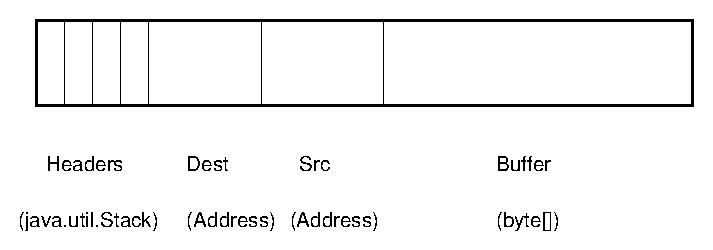
\epsfig{file=figs/Message.eps,width=.55\textwidth}}
       \caption{Structure of a message}
       \label{MessageFig}
  \end{figure}

  A message is similar to an IP packet and consists of the payload (a byte buffer)
  and the addresses of the sender and receiver (as Addresses). Any message put on the
  network can be routed to its destination (receiver address), and replies can be
  returned to the sender's address.

  A message usually does not need to fill in the sender's address when sending a
  message; this is done automatically by the protocol stack before a message is
  put on the network. However, there may be cases, when the sender of a message
  wants to give an address different from its own, so that for example, a response
  should be returned to some other member.

  The destination address (receiver) can be an Address, denoting the address of a
  member, determined e.g. from a message received previously, or it can be {\tt
  null}, which means that the message will be sent to all members of the group. A
  typical multicast message, sending string {\tt "Hello"} to all members would
  look like this:

  \begin{small}
  \begin{verbatim}
  Message msg=new Message(null, null, "Hello".getBytes());
  channel.send(msg);
  \end{verbatim}
  \end{small}



  \section{View} \label{View}

  A View ({\tt View}) is a list of the current members of a group. It consists of a
  {\tt ViewId}, which uniquely identifies the view (see below), and a list of
  members. Views are set in a channel automatically by the underlying protocol stack
  whenever a new member joins or an existing one leaves (or crashes). All members of
  a group see the same sequence of views.

  Note that there is a comparison function which orders all the members of a group
  in the same way. Usually, the first member of the list is the {\em coordinator}
  (the one who emits new views). Thus, whenever the membership changes, every member
  can determine the coordinator easily and without having to contact other members.
  
  The code below shows how to send a (unicast) message to the first member of a view
  (error checking code omitted):

  \begin{small}
  \begin{verbatim}
  View    myview=channel.getView();
  Address first=myview.getMembers().first();
  Message msg=new Message(first, null, "Hello world");
  channel.send(msg);
  \end{verbatim}
  \end{small}


  Whenever an application is notified that a new view has been installed (e.g. by
  {\tt MembershipListener.viewAccepted()} or {\tt Channel.receive()}), the view is
  already set in the channel. For example, calling {\tt Channel.getView()} in a {\tt
  viewAccepted()} callback would return the same view (or possibly the next one in
  case there has already been a new view !).

    \subsection{ViewId} \label{ViewId}

    The ViewId is used to uniquely number views. It consists of the address of the
    view creator and a sequence number. ViewIds can be compared for equality and put
    in a hashtable as they implement equals() and hashCode() methods.


    \subsection{MergeView} \label{MergeView}

    Whenever a group splits into subgroups, e.g. due to a network partition, and
    later the subgroups merge back together, a MergeView instead of a View will be
    received by the application. The MergeView class is a subclass of View and
    contains as additional instance variable the list of views that were merged. As
    an example if the group denoted by view {\tt V1:(p,q,r,s,t)} split into subgroups
    {\tt V2:(p,q,r)} and {\tt V2:(s,t)}, the merged view might be {\tt
    V3:(p,q,r,s,t)}. In this case the MergeView would contains a list of 2 views:
    {\tt V2:(p,q,r)} and {\tt V2:(s,t)}.





  \section{Membership} \label{Membership}

  This class can be used for keeping rack of members instead of a Vector class. It
  adds several functions, such as duplicate elimination, merging with other
  Membership instances and sorting.


  
  \section{Channel} \label{Channels}

  In order to join a group and send messages, a process has to create a channel. A
  channel is like a socket. When a client connects to a channel, it gives the the
  name of the group it would like to join. Thus, a channel is (in its connected
  state) always associated with a particular group. The protocol stack takes care
  that channels with the same group name find each other: whenever a client connects
  to a channel given group name G, then it tries to find existing channels with the
  same name, and joins them, resulting in a new view being installed (which contains
  the new member). If no members exist, a new group will be created.

  A state transition diagram for the major states a channel can assume are shown in
  fig. \ref{ChannelStatesFig}.

  \begin{figure}[htb]
      \center{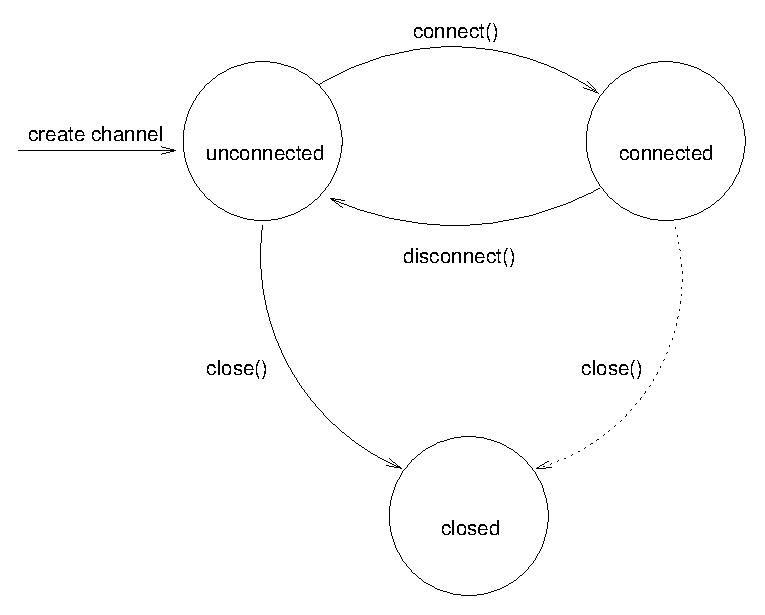
\epsfig{file=figs/ChannelStates.eps,width=.5\textwidth}}
      \caption{Channel states}
      \label{ChannelStatesFig}
  \end{figure}

  When a channel is first created, it is in the unconnected state. An attempt to
  perform certain operations which are only valid in the connected state
  (e.g. send/receive messages) will result in an exception. After a successful
  connection by a client, it moves to the connected state. Now channels will
  receive messages, views and suspicions from other members and may send messages
  to other members or to the group. Getting the local address of a channel is
  guaranteed to be a valid operation in this state (see below). When the channel is
  disconnected, it moves back to the unconnected state. Both a connected and
  unconnected channel may be closed, which makes the channel unusable for further
  operations. Any attempt to do so will result in an exception. When a channel is
  closed directly from a connected state, it will first be disconnected, and then
  closed.

  The methods available for creating and manipulating channels are discussed now.


    \subsection{Creating a channel}

    A channel can be created in two ways: an instance of a subclass of {\tt Channel}
    is created directly using its public constructor (e.g. {\tt new JChannel()}),
    or a channel factory is created, which -- upon request -- creates instances of
    channels. We will only look at the first method of creating channel: by direct
    instantiation. Note that instantiation may differ between the various channel
    implementations. As example we will look at {\tt JChannel}.

    The public constructor of {\tt JChannel} looks as follows:

    \begin{small}
    \begin{verbatim}
    public JChannel(Object properties) throws ChannelException {}
    \end{verbatim}
    \end{small}

    It creates an instance of {\tt JChannel}. The {\tt properties} argument defines
    the composition of the protocol stack (number and type of layers, parameters for
    each layer, and their order). For JChannel, this has to be a String (see
    \ref{ChannelProperties} for how to define one's own properties string). An
    example of a channel creation is
    
    \begin{small}
    \begin{verbatim}
    String props="UDP(mcast_addr=228.1.2.3;mcast_port=45566;ip_ttl=32):" +
        "PING(timeout=3000;num_initial_members=6):" +
        "FD(timeout=5000):" +
        "VERIFY_SUSPECT(timeout=1500):" +
        "pbcast.STABLE(desired_avg_gossip=10000):" +
        "pbcast.NAKACK(gc_lag=10;retransmit_timeout=3000):" +
        "UNICAST(timeout=5000;min_wait_time=2000):" +
        "FRAG:" +
        "pbcast.GMS(initial_mbrs_timeout=4000;join_timeout=5000;" +
        "join_retry_timeout=2000;shun=false;print_local_addr=false)";
    JChannel channel;
    try {
        channel=new JChannel(props);
    }
    catch(Exception ex) {
        // channel creation failed
    }
    \end{verbatim}
    \end{small}

    The argument is a colon-delimited string of protocols, specified from bottom to
    top (left to right). The example properties argument will be used to create a
    protocol stack that uses IP Multicast (UDP) as bottom protocol, the PING protocol
    to locate the initial members, FD for failure detection, VERIFY\_SUSPECT for
    double-checking of suspected members, STABLE for garbage collection of messages
    received by all members, NAKACK for lossless delivery of multicast messages,
    UNICAST for lossless delivery of unicast messages and GMS for group membership
    (handling of join or leave requests).

    If the properties argument is null, the default properties will be used. An
    exception will be thrown if the channel cannot be created. Possible causes
    include protocols that were specified in the property argument, but were not
    found, or wrong parameters to protocols.



    \subsection{Channel properties} \label{ChannelProperties}

    A property string consists of a number of properties separated by colons:

    \begin{small}
    \begin{verbatim}
    "<prop1>(arg1=val1):<prop2>(arg1=val1;arg2=val2):<prop3>:<propn>"
    \end{verbatim}
    \end{small}

    Each property relates directly to a protocol layer, which is implemented as a
    Java class. When a protocol stack is to be created based on the above property
    string, the first property becomes the bottom-most layer, the second one will be
    placed on the first, etc: the stack is created from the bottom to the top, as the
    string is parsed from left to right. Each property has to be the name of a Java
    class that resides in the {\tt org.javagroups.stack.protocols} package. Note that
    only the base name has to be given, not the fully specified class name ({\tt UDP}
    instead of {\tt org.javagroups.stack.protocols.UDP}).

    Each layer may have zero or more arguments, which are specified as a list of
    name/value pairs in parentheses directly after the property. In the example
    above, the first protocol layer has 1 argument, the second 2, the third
    none. When a layer is created these properties (if there are any) will be set in
    a protocol, thus configuring the protocol stack according to the channel creator.

    As an example the property string below instructs JavaGroups to create a
    JChannel with protocols {\tt UDP}, {\tt PING}, {\tt FD} and {\tt GMS}:


    \begin{small}
    \begin{verbatim}
    "UDP(mcast_addr=228.10.9.8;mcast_port=5678):PING:FD:GMS"
    \end{verbatim}
    \end{small}

    The {\tt UDP} protocol layer is at the bottom of the stack, and it should use
    mcast address {\tt 228.10.9.8.} and port {\tt 5678} rather than the default IP
    multicast address and port. Property {\tt UDP} refers to a class {\tt
    org.javagroups.stack.protocols.UDP}, which is subsequently loaded and an instance
    of which is created as protocol layer. If any of these classes are not found, an
    exception will be thrown and the construction of the stack will be aborted.

    {\em Note that all members in a group have to have the same protocol stack.}



    \subsection{Setting options} \label{SettingOptions}

    A number of options can be set in a channel. To do so, the following method is
    used:

    \begin{small}
    \begin{verbatim}
    public void setOpt(int option, Object value);
    \end{verbatim}
    \end{small}

    Arguments are the options number and a value. The following options are currently
    recognized:

    \begin{description}

    \item[Channel.VIEW] The argument must be a boolean value {\tt Boolean}. If true,
	                views will be received (default is true). If false, no views
	                will be received.

    \item[Channel.SUSPECT] The argument is also a boolean object. If set to true,
	                   suspicion messages will be received, otherwise not
	                   (default is false).

    \item[Channel.BLOCK] The argument is a boolean object. If true, block messages
	                 will be received. If this option is set to true, views will
	                 also be set to true. Default is false.

    \item[Channel.LOCAL] Local delivery. The argument is a boolean value. If set to
	                 true, a member will receive all messages it sent to
	                 itself. Otherwise, all messages sent by itself will be
	                 discarded. This option allows to send messages to the group,
	                 without receiving a copy. Default is true (members will
	                 receive their own copy of messages multicast to the group).

    \item[Channel.GET\_STATE\_EVENTS] Reception of {\tt GetStateEvent}s. If this option is
	  	              turned off, then the group's state may be retrieved,
	  	              but this member will not respond to requests for its
	  	              state (client role).

    \end{description}

    The equivalent method to get options is {\tt getOpt()}:

    \begin{small}
    \begin{verbatim}
    public Object getOpt(int option);
    \end{verbatim}
    \end{small}

    Given an option, the current value of the option is returned.




    \subsection{Connecting to a channel}

    When a client wants to join a group, it {\em connects} to a channel giving the
    name of the group to be joined:

    \begin{small}
    \begin{verbatim}
    public void connect(String groupname) throws ChannelClosed;
    \end{verbatim}
    \end{small}

    The group address is a string, naming the group to be joined. All channels that
    are connected to the same group (same name) form a group. Messages multicast on
    any channel in the group will be received by all members (including the one who
    sent it\footnote{Local delivery can be turned on/off using {\tt setOpt()}.}).

    The method returns as soon as the group has been joined successfully. If the
    channel is in the closed state (see fig. \ref{ChannelStatesFig}), an exception
    will be thrown. If there are no other members, i.e. no other client has connected
    to a group with this name, then a new group is created and the member joined. The
    first member of a group becomes its {\em coordinator}. A coordinator is in charge
    of multicasting new views whenever the membership changes\footnote{This is
    managed internally however, and an application programmer does not need to be
    concerned about it.}.


    \subsection{Getting the local address and the group name}

    Method {\tt getLocalAddress()} returns the local address of the channel. In the
    case of {\tt JChannel}, the local address is generated by the bottom-most layer
    of the protocol stack when the stack is connected to. That means that --
    depending on the channel implementation -- the local address may or may not be
    available when a channel is in the unconnected state.

    \begin{small}
    \begin{verbatim}
    public Address getLocalAddress();
    \end{verbatim}
    \end{small}

    Method {\tt getChannelName()} returns the name of the group in which the channel
    is a member:

    \begin{small}
    \begin{verbatim}
    public String getChannelName();
    \end{verbatim}
    \end{small}

    Again, the result is undefined if the channel is in the unconnected or closed
    state.



    \subsection{Getting the current view}

    The following method can be used to get the current view of a channel:
	
    \begin{small}
    \begin{verbatim}
    public View getView();
    \end{verbatim}
    \end{small}

    This method does {\em not} retrieve a new view (message) from the channel, but
    only returns the current view of the channel. The current view is updated every
    time a view message is received: when method {\tt receive()} is called, and the
    return value is a view, before the view is returned, it will be installed in the
    channel, i.e. it will become the current view.

    Calling this method on an unconnected or closed channel is implementation
    defined. A channel may return null, or it may return the last view it knew of.




    \subsection{Sending a message}

    Once the channel is connected, messages can be sent using the send() methods:

    \begin{small}
    \begin{verbatim}
    public void send(Message msg) throws ChannelNotConnected, ChannelClosed;
    public void send(Address dst, Address src, Object obj) throws ChannelNotConnected, ChannelClosed;
    \end{verbatim}
    \end{small}

    The first {\tt send()} method has only one argument, which is the message to be
    sent. The message's destination should either be the address of the receiver
    (unicast) or null (multicast). When it is null, the message will be sent to all
    members of the group (including itself). The source address may be null; if it
    is, it will be set to the channel's address (so that recipients may generate a
    response and send it back to the sender).

    The second send() method is a helper method and uses the former method
    internally. It requires the address of receiver and sender and an object (which
    has to be serializable), constructs a Message and sends it.

    If the channel is not connected, or was closed, an exception will be thrown upon
    attempting to send a message.


    Here's an example of sending a (multicast) message to all members of a group:
    
    \begin{small}
    \begin{verbatim}
    Hashtable data;  // any serializable data
    try {
        channel.send(null, null, data);
    }
    catch(Exception ex) {
        // handle errors
    }
    \end{verbatim}
    \end{small}

    The null value as destination address means that the message will be sent to all
    members in th group. The sender's address will be filled in by the bottom-most
    protocol. The payload is a hashtable, which will be serialized into the message's
    buffer and unserialized at the receiver's end. Alternatively, any other means of
    generating a byte buffer and setting the message's buffer to it (e.g. using
    Message.setBuffer()) would also work.


    Here's an example of sending a (unicast) message to the first member
    (coordinator) of a group:

    \begin{small}
    \begin{verbatim}
    Address   receiver;
    Message   msg;
    Hashtable data;
    try {
        receiver=channel.getView().getMembers().first();
        channel.send(receiver, null, data);
    }
    catch(Exception ex) {
        // handle errors
    }
    \end{verbatim}
    \end{small}

    It creates a Message with a specific address for the receiver (the first member
    of the group). Again, the sender's address can be left null as it will be filled
    in by the bottom-most protocol.

	
    \subsection{Receiving a message}

    Method {\tt receive()} is used to receive messages, views, suspicions and blocks:	

    \begin{small}
    \begin{verbatim}
    public Object receive(long timeout) throws ChannelNotConnected, ChannelClosed, Timeout;
    \end{verbatim}
    \end{small}

    A channel receives messages asynchronously from the network and stores them in a
    queue. When receive() is called, the next available message from the top of that
    queue is removed and returned. When there are no messages on the queue, the
    method will block. If {\tt timeout} is greater than 0, it will wait the specified
    number of milliseconds for a message to be received, and throw a {\tt
    TimeoutException} exception if none was received during that time. If the timeout
    is 0 or negative, the method will wait indefinitely for the next available
    message.

    Depending on the channel options (see \ref{SettingOptions}), the following
    types of objects may be received:

    \begin{description}

    \item[Message] A regular message. To send a response to the sender, a new
	           message can be created. Its destination address would be the
	           received message's source address. Method {\tt
	           Message.makeReply()} is a helper method to create a response.

    \item[View] A view change, signalling that a member has joined, left or
	        crashed. The application may or may not perform some action upon
	        receiving a view change (e.g. updating a GUI object of the
	        membership, or redistributing a load-balanced collaborative task
	        to all members). Note that a longer action, or any action that
	        blocks should be performed in a separate thread.
		A {\tt MergeView} will be received when 2 or more subgroups merged
	        into one (see \ref{MergeView} for details). Here, a possible state
	        merge by the application needs to be done in a separate thread.

    \item[SuspectEvent] Notification of a member that is suspected. Method {\tt
	                SuspectEvent.getMember()} retrieves the address of the
	                suspected member. Usually this message will be followed
	                by a view change.

    \item[BlockEvent] The application has to stop sending messages {\em until a new
	              view has been received}. It is used to synchronize messages
	              between views, so that all messages are received in the view in
	              which they are sent. When the application has stopped sending
	              messages, it needs to acknowledge this message with a {\tt
	              Channel.blockOk()} method. Messages of this type are not
	              usually enabled on a channel (see \ref{SettingOptions}),
	              therefore an application will not receive blocks at all. In
	              case they {\em are} enabled, {\tt blockOk()} has been invoked,
	              and the application sends a message before having received the
	              next view, the view in which the message will be delivered is
	              not determined: it may be the next view, or any the message may
	              even be discarded ! When blocks are not enabled, the view in
	              which a message will be delivered, is not determined (but no
	              message will be discarded !)

    \item[GetStateEvent] Received when the application's current state should be
                         saved (for a later state transfer. A {\em copy} of the
                         current state should be made (possibly wrapped in a {\tt
                         synchronized} statement and returned calling method {\tt
                         Channel.returnState()}. If state transfer events are not
                         enabled on the channel (default), then this event will never
                         be received. This message will only be received with the
                         Virtual Synchrony suite of protocols (see the Programmer's
                         Guide).

    \item[SetStateEvent] Received as response to a {\tt getState(s)} method
	                 call. The argument contains the state of a single member
			 ({\tt byte[]}) or of all members ({\tt Vector}). Since
			 the state of a single member could also be a vector,
			 the interpretation of the argument is left to the
			 application.

    \end{description}

    The caller has to check the type of the object returned. This can be done using
    the {\tt instanceof} operator, as follows:


    \begin{small}
    \begin{verbatim}
    Object  obj;
    Message msg;
    View    v;
    obj=channel.receive(0); // wait forever
    if(obj instanceof Message)
        msg=(Message)obj;
    else if(obj instanceof View)
        v=(View)obj;
    else
       ; // don't handle suspicions or blocks
    \end{verbatim}
    \end{small}

    If for example views, suspicions and blocks are disabled, then the caller is
    guaranteed to only receive return values of type {\tt Message}. In this case,
    the return value can be cast to a {\tt Message} directly, without using the {\tt
    instanceof} operator.

    If the channel is not connected, or was closed, a corresponding exception
    will be thrown.

    The example below shows how to retrieve the "Hello world" string from a message:
    
    \begin{small}
    \begin{verbatim}
    Message msg; // received above
    String  s;
    try {
        s=(String)msg.getObject(); // error if object not Serializable
        // alternative: s=new String(msg.getBuffer());
    }
    catch(Exception ex) {
        // handle errors, e.g. casting error above)
    }
    \end{verbatim}
    \end{small}
	
    The Message.getObject() method retrieves the message's byte buffer, converts it
    into a (serializable) object and returns the object.


    \subsection{Peeking at a message}

    Instead of removing the next available message from the channel, {\tt peek()}
    just returns a reference to the next message, but does not remove it. This is
    useful when one has to check the type of the next message, e.g. whether it is a
    regular message, or a view change. The signature of this method is not shown
    here, it is the same as for {\tt receive()}.



    \subsection{Getting the group's state} \label{GetState}

    A newly joined member may wish to retrieve the state of the group before starting
    work. This is done calling either {\tt getState()} of {\tt getStates()}. The
    first method returns the state of one member (in most cases, of the oldest
    member, the coordinator) whereas the latter returns the states of all
    members. This method returns true or false, depending on whether a valid state
    could be retrieved. For example, if a member is a singleton, then calling this
    method would always return false\footnote{A member will {\em never} retrieve the
    state from itself !}.

    The actual state is returned as the return value of one of the subsequent {\tt
    receive()} calls, in the form of a {\tt SetStateEvent} object. If {\tt getState(s)}
    returned true, then a valid state (non-null) will be returned, otherwise a null
    state will be returned. Alternatively if an application uses MembershipListener
    (see \ref{MembershipListener}) instead of pulling messages from a channel, the
    {\tt getState()} method will be invoked and a copy of the current state should
    be returned. By the same token, setting a state would be accomplished by
    JavaGroups calling the {\tt setState()} method of the state fetcher.
    
    The reason for not directly returning the state as a result of {\tt getState()} is
    that the state has to be returned in the correct position relative to other
    messages. Returning it directly would violate the FIFO properties of a channel,
    and state transfer would not be correct.

    The following code fragment shows how a group member participates in state
    transfers:

    \begin{small}
    \begin{verbatim}
    channel=new JChannel("UDP:PING:FD:GMS:STATE_TRANSFER:QUEUE");
    channel.setOpt(Channel.GET_STATE_EVENTS, new Boolean(true));
    channel.connect("TestChannel");
    boolean rc=channel.getState(5000);

    ...

    Object state, copy;
    Object ret=channel.receive(0);
    if(ret instanceof Message)
        ;
    else if(ret instanceof GetStateEvent) {
        copy=copyState(state); // make a copy so that other msgs don't change the state
        channel.returnState(Util.objectToByteBuffer(copy));
    }
    else if(ret instanceof SetStateEvent) {
        SetStateEvent e=(SetStateEvent)ret;
        // set state from ret.GetArg();
    }
    \end{verbatim}
    \end{small}


    A JChannel has to be created whose stack includes the {\tt STATE\_TRANSFER} or
    {\tt pbcast.STATE\_TRANSFER} protocols (see \ref{Advanced}). Option {\tt
    GET\_STATE\_EVENTS} should be enabled, as the channel might probably want to
    return its current state if asked. Method {\tt getState()} subsequently asks the
    channel to return the current state. If there is a current state (there may not
    be any other members in the group !), then true is returned. In this case, one of
    the subsequent {\tt receive()} method invocations on the channel will return a {\tt
    SetStateEvent} object which contains the current state. In this case, the caller
    sets its state to the one received from the channel.

    If state transfer events are enabled, then {\tt receive()} might return a {\tt
    GetStateEvent} object, requesting the state of the member to be returned. In this
    case, {\em a copy of the current state should be made} and returned using {\tt
    JChannel.returnState()}. It is important to a) synchronize access to the state when
    returning it since other accesses may modify it while it is being returned and b)
    make a copy of the state since other accesses after returning the state may still
    be able to modify it ! This is possible because the state is not immediately
    returned, but travels down the stack (in the same address space), and a reference
    to it could still alter it.

	

    The details of state transfer as implemented in JavaGroups are discussed in the
    Programmer's Guide.






    \subsection{Disconnecting from a channel}

    Disconnecting from a channel is done using the following method:

    \begin{small}
    \begin{verbatim}
    public void disconnect();
    \end{verbatim}
    \end{small}

    It will have no effect if the channel is already in the disconnected or closed
    state. If connected, it will remove itself from the group membership. This is
    done (transparently for a channel user) by sending a leave request to the current
    coordinator. The latter will subsequently remove the channel's address from its
    local view and send the new view to all remaining members.

    After a successful disconnect, the channel will be in the unconnected state, and
    may subsequently be re-connected to.



    \subsection{Closing a channel}

    To destroy a channel instance (destroy the associated protocol stack, and release
    all resources), method {\tt close()} is used:

    \begin{small}
    \begin{verbatim}
    public void close();
    \end{verbatim}
    \end{small}

    It moves the channel to the closed state, in which no further operations are
    allowed (most throw an exception when invoked on a closed channel). In this
    state, a channel instance is not considered used any longer by an application and
    -- when the reference to the instance is reset -- the channel essentially only
    lingers around until it is garbage collected by the Java runtime system.





    






